\chapter{From Metric to Topology}

We will study global properties of a geometric object, i.e., the distrance between 2 points in an object is totally ignored. For example, the objects shown below are essentially invariant under a certain kind of transformation:

\begin{center}
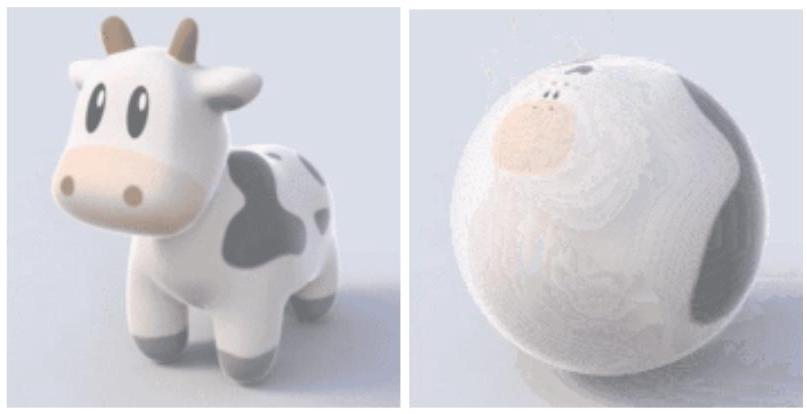
\includegraphics[width=0.5\textwidth]{images/ch1_cow.jpg}
\end{center}
\hspace*{3em} 

Another example is that the coffee cup and the donut have the same topology:

\begin{center}
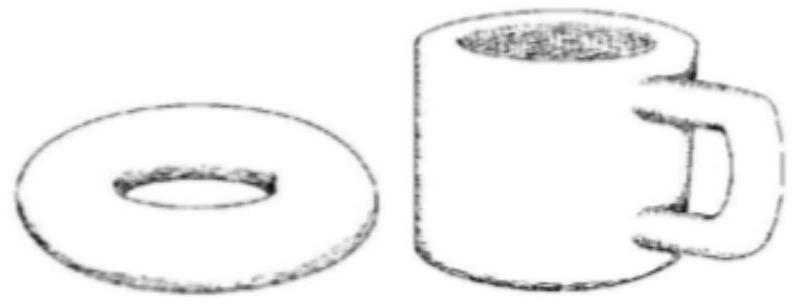
\includegraphics[width=0.5\textwidth]{images/ch1_donutmug.jpg}
\end{center}

However, the two objects below have the intrinsically different topologies:

\begin{center}
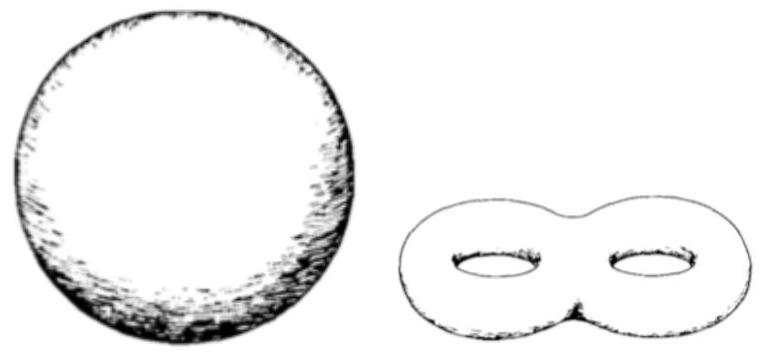
\includegraphics[width=0.5\textwidth]{images/ch1_twoholes.jpg}
\end{center}

In this course, we will study the phenomenon described above mathematically.

\section{Metric Spaces}
In this section, we will study a special kind of topological space.

\begin{definition}[Metric Space] \label{def:metric_space} A metric space \((X,d)\) is a non-empty set endowed with a function (distance function) \(d : X \times  X \rightarrow  \mathbb{R}\) such that

1. \(d\left( {\mathbf{x},\mathbf{y}}\right)  \geq  0\) for \(\forall \mathbf{x},\mathbf{y} \in  X\) with equality iff \(\mathbf{x} = \mathbf{y}\)

2. \(d\left( {\mathbf{x},\mathbf{y}}\right)  = d\left( {\mathbf{y},\mathbf{x}}\right)\)

3. \(d\left( {\mathbf{x},\mathbf{z}}\right)  \leq  d\left( {\mathbf{x},\mathbf{y}}\right)  + d\left( {\mathbf{y},\mathbf{z}}\right)\) (triangle inequality)
\end{definition}

\begin{example} \begin{enumerate}
    \item Let \(X = {\mathbb{R}}^{n}\). Then the distance functions:
\[
{d}_{2}\left( {\mathbf{x},\mathbf{y}}\right)  = \sqrt{\mathop{\sum }\limits_{{i = 1}}^{n}{\left( {x}_{i}- {y}_{i}\right) }^{2}}
\quad, \quad {d}_{\infty }\left( {\mathbf{x},\mathbf{y}}\right)  = \mathop{\max }\limits_{{i = 1,\ldots,n}}\left| {{x}_{i}- {y}_{i}}\right|
\]
define two different metric spaces of the same set $X$.

\item Let \(X\) be any set, and define the discrete metric
\[
d\left( {\mathbf{x},\mathbf{y}}\right)  = \left\{  \begin{array}{ll} 0, & \text{ if }x = y \\  1, & \text{ if }x \neq  y \end{array}\right.
\]
\end{enumerate}
(Homework Show that (1) and (2) defines a metric.)
\end{example}

\begin{definition}[Open Ball] Let $(X,d)$ be a metric space. An open ball of radius \(r\) centered at \(\mathbf{x} \in  X\) is the set
\[
{B}_{r}\left( \mathbf{x}\right)  = \{ \mathbf{y} \in  X \mid  d\left( {\mathbf{x},\mathbf{y}}\right)  < r\}
\]
\end{definition}

\begin{example} \begin{enumerate}
    \item The set \({B}_{1}\left( {0,0}\right)\) defines an open ball under the metric \(\left( {X = {\mathbb{R}}^{2},{d}_{2}}\right)\), or the metric \(\left( {X = {\mathbb{R}}^{2},{d}_{\infty }}\right)\). The corresponding diagram is shown below:
\begin{center}
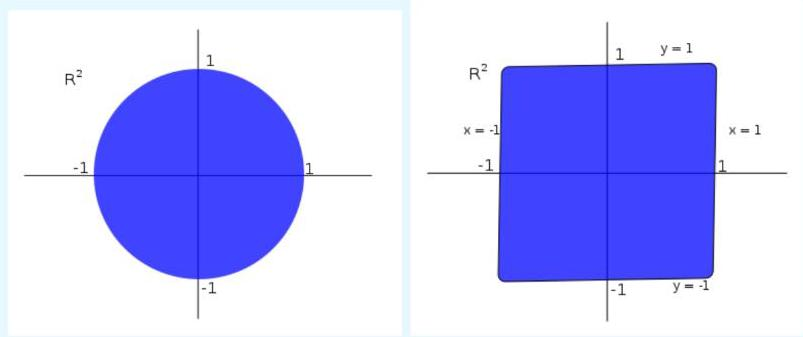
\includegraphics[width=0.6\textwidth]{images/ch1_ball_square.jpg}
\end{center}

\item Under the discrete metric \(({X = {\mathbb{R}}^{2}}, d_{discrete})\), the open ball \({B}_{1}\left( {{\bf x},0}\right)\) is a single point.
\end{enumerate}
\end{example}

\begin{definition}[Open Set] \label{def:open_set} Let \(X\) be a metric space, \(U \subseteq  X\) is an open set in \(X\) if \(\forall u \in  U\), there exists \({\epsilon }_{u} > 0\) such that \({B}_{{\epsilon }_{u}}\left( u\right)  \subseteq  U\).
\end{definition}

Now we get our first taste of topology- the main subject we are studying in this course:
\begin{definition} The \emph{topology} $(X, \mathcal{T})$ induced from a metric space $(X, d)$ is the collection of all open sets 
$$\mathcal{T} := \{ U \subset X\ |\ U\ \text{is open}\}$$ 
in $(X, d)$ (by convention, we decree that the empty set \(\varnothing \in \mathcal{T}\) is open).
\end{definition}

\begin{proposition} All open balls \({B}_{r}\left( \mathbf{x}\right)\) are open in $(X, d)$, i.e. ${B}_{r}\left( \mathbf{x}\right) \in \mathcal{T}$.
\end{proposition}

\begin{proof} Consider the example \(X = \mathbb{R}\) with metric \({d}_{2}\). Therefore \({B}_{r}\left( x\right)  = \left( {x- r,x + r}\right)\). Take \(\mathbf{y} \in  {B}_{r}\left( \mathbf{x}\right)\) such that \(d\left( {\mathbf{x},\mathbf{y}}\right)  = q < r\) and consider \({B}_{\left( {r- q}\right) /2}\left( \mathbf{y}\right)\) : for all \(z \in  {B}_{\left( {r- q}\right) /2}\left( \mathbf{y}\right)\), we have
\[
d\left( {\mathbf{x},\mathbf{z}}\right)  \leq  d\left( {\mathbf{x},\mathbf{y}}\right)  + d\left( {\mathbf{y},\mathbf{z}}\right)  < q + \frac{r- q}{2} < r,
\]
which implies \(z \in  {B}_{r}\left( x\right)\).
\end{proof}

\begin{proposition} \label{prop:open_metric_space} Let $(X, d)$ be a metric space, and \(\mathcal{T}\) is the topology induced from $(X, d)$, then
\begin{enumerate}
    \item Let \(\left\{  {{G}_{\alpha } \mid  \alpha  \in  \mathcal{A}}\right\}\) be such that \({G}_{\alpha } \in  \mathcal{T}\) for all $\alpha \in \mathcal{A}$, then \[\mathop{\bigcup }\limits_{{\alpha  \in  \mathcal{A}}}{G}_{\alpha } \in  \mathcal{T}\].
\item let \({G}_{1},\ldots,{G}_{n} \in  \mathcal{T}\), then 
\[\mathop{\bigcap }\limits_{{i = 1}}^{n}{G}_{i} \in  \mathcal{T}\]
that is, the finite intersection of open sets is open.
\end{enumerate}
\end{proposition}

\begin{proof} \begin{enumerate}
    \item Take \(x \in  \mathop{\bigcup }\limits_{{\alpha  \in  \mathcal{A}}}{G}_{\alpha }\), then \(x \in  {G}_{\beta }\) for some \(\beta  \in  \mathcal{A}\). Since \({G}_{\beta }\) is open, there exists \({\epsilon }_{x} > 0\) such that
\[
{B}_{{\epsilon }_{x}}\left( x\right)  \subseteq  {G}_{\beta } \subseteq  \mathop{\bigcup }\limits_{{\alpha  \in  \mathcal{A}}}{G}_{\alpha }
\]

\item Take \(x \in  \mathop{\bigcap }\limits_{{i = 1}}^{n}{G}_{i}\), i.e., \(x \in  {G}_{i}\) for \(i = 1,\ldots,n\), i.e., there exists \({\epsilon }_{i} > 0\) such that \({B}_{{\epsilon }_{i}}\left( x\right)  \subseteq  {G}_{i}\) for \(i = 1,\ldots,n\). Take \(\epsilon  = \min \left\{  {{\epsilon }_{1},\ldots,{\epsilon }_{n}}\right\}\), which implies
\[
{B}_{\epsilon }\left( x\right)  \subseteq  {B}_{{\epsilon }_{i}}\left( x\right)  \subseteq  {G}_{i},\forall i
\]
which implies \({B}_{\epsilon }\left( x\right)  \subseteq  \mathop{\bigcap }\limits_{{i = 1}}^{n}{G}_{i}\)
\end{enumerate}
\end{proof}

\begin{exercise}
\begin{enumerate}
    \item Let \({\mathcal{T}}_{2},{\mathcal{T}}_{\infty }\) be topologies induced from the metrics \({d}_{2},{d}_{\infty }\) in \({\mathbb{R}}^{2}\). Show that \({\mathcal{T}}_{2} = {\mathcal{T}}_{\infty }\), i.e., every open set in \(\left( {{\mathbb{R}}^{2},{d}_{2}}\right)\) is open in \(\left( {{\mathbb{R}}^{2},{d}_{\infty }}\right)\), and every open set in \(\left( {{\mathbb{R}}^{2},{d}_{\infty }}\right)\) is open in \(\left( {{\mathbb{R}}_{2},{d}_{2}}\right)\).

\item Let \(\mathcal{T}\) be the topology induced from the discrete metric \(\left( {X,{d}_{\text{ discrete }}}\right)\). What is \(\mathcal{T}\)?
\end{enumerate} 
\end{exercise}

({\it Hint:} for (1), show that an open ball in \({d}_{2}\)-metric is open in \({d}_{\infty }\); any open set in \({d}_{2}\)-metric is open in \({d}_{\infty }\); then switch the roles of \({d}_{2}\) and \({d}_{\infty }\)).


\section{Understanding Metric Spaces via Topology}
In a standard second course of analysis, one studies various properties of metric spaces $(X,d)$ such as closedness, compactness, continuous maps, etc. In this section, we will re-define these familiar notions by just using the topology $\mathcal{T}$ of $X$.

\subsection{Closed sets}
\begin{definition}[Closed] A subset \(V \subseteq  X\) is closed if \(X \smallsetminus  V\) is open.
\end{definition}

\begin{example} Under the metric space \(\left( {\mathbb{R},{d}_{1}}\right)\),
\[
\mathbb{R} \smallsetminus  \left\lbrack  {b,a}\right\rbrack   = \left( {a,\infty }\right) \bigcup \left( {-\infty,b}\right) \text{ is open } \Rightarrow  \left\lbrack  {b,a}\right\rbrack  \text{ is closed }
\]

1. \(\varnothing,X\) is closed in \(X\)

2. If \({F}_{\alpha }\) is closed in \(X\), so is \(\mathop{\bigcap }\limits_{{\alpha  \in  A}}{F}_{\alpha }\).

3. If \({F}_{1},\ldots,{F}_{k}\) is closed, so is \(\mathop{\bigcup }\limits_{{i = 1}}^{k}{F}_{i}\).
\end{example}

\begin{proof} 1. Note that \(X\) is open in \(X\), which implies \(\varnothing  = X \smallsetminus  X\) is closed in \(X\); Similarly, \(\varnothing\) is open in \(X\), which implies \(X = X \smallsetminus  \varnothing\) is closed in \(X\);

2. The set \({F}_{\alpha }\) is closed implies there exists open \({U}_{\alpha } \subseteq  X\) such that \({F}_{\alpha } = X \smallsetminus  {U}_{\alpha }\). By De Morgan's Law,
\[
\mathop{\bigcap }\limits_{{\alpha  \in  A}}{F}_{\alpha } = \mathop{\bigcap }\limits_{{\alpha  \in  A}}\left( {X \smallsetminus  {U}_{\alpha }}\right)  = X \smallsetminus  \left( {\mathop{\bigcup }\limits_{{\alpha  \in  A}}{U}_{\alpha }}\right).
\]

By part (1) in \autoref{prop:open_metric_space}, the set \(\mathop{\bigcup }\limits_{{\alpha  \in  A}}{U}_{\alpha }\) is open, which implies \(\mathop{\bigcap }\limits_{{\alpha  \in  A}}{F}_{\alpha }\) is closed.

3. The result follows from part (2) in \autoref{prop:open_metric_space} by taking complements. We illustrate examples where open set is used to define convergence and continuity.
\end{proof}

\subsection{Convergence of sequences}
Recall that in the case of metric space $(X, d)$, a sequence of $X$ \(\left\{  {x}_{n}\right\} \rightarrow  x\) converges to $x \in X$ means
\[
\forall \varepsilon  > 0,\exists N\text{ such that }d\left( {{x}_{n},x}\right)  < \varepsilon,\forall n \geq  N\text{. }
\]
We will study the convergence by using $\mathcal{T}$ instead of $d$.

\begin{proposition} Let \((X,d)\) be a metric space, then \(\left\{  {x}_{n}\right\}  \rightarrow  x\) if and only if for \(\forall\) open set \(U \ni  x\), there exists \(N\) such that \({x}_{n} \in  U\) for \(\forall n \geq  N\).
\end{proposition}

\begin{proof} Necessity: Since \(U \ni  x\) is open, there exists \(\varepsilon  > 0\) such that \({B}_{\varepsilon }\left( x\right)  \subseteq  U\).
Since \(\left\{  {x}_{n}\right\}   \rightarrow  x\), there exists \(N\) such that \(d\left( {{x}_{n},x}\right)  < \varepsilon\), i.e., \({x}_{n} \in  {B}_{\varepsilon }\left( x\right)  \subseteq  U\) for \(\forall n \geq  N\).

Sufficiency: Let \(\varepsilon  > 0\) be given. Take the open set \(U = {B}_{\varepsilon }\left( x\right)  \ni  x\), then there exists \(N\)
\end{proof}

\subsection{Continuity}
\begin{definition}[Continuity] Let $(X, d)$ and \(\left( {Y,\rho }\right)\) be given metric spaces. Then \(f : X \rightarrow  Y\) is continuous at \({x}_{0} \in  X\) if
\[
\forall \varepsilon  > 0,\exists \delta  > 0\text{ such that }d\left( {x,{x}_{0}}\right)  < \delta  \Rightarrow  \rho \left( {f\left( x\right),f\left( {x}_{0}\right) }\right)  < \varepsilon \text{. }
\]
The function \(f\) is continuous on \(X\) if \(f\) is continuous for all \({x}_{0} \in  X\).
\end{definition}

As before, we now get rid of metrics to study continuity:
\begin{proposition} \label{prop:metric_cont_map} Let $X, Y$ be metric spaces, and $f:X \to Y$ is a function. 

\begin{enumerate}
    \item The function \(f\) is continuous at \(x\) if and only if for all open \(U \ni  f\left( x\right)\), there exists \(\delta  > 0\) such that the set \(B\left( {x,\delta }\right)  \subseteq  {f}^{-1}\left( U\right)\).

\item The function \(f\) is continuous on \(X\) if and only if \({f}^{-1}\left( U\right)\) is open in \(X\) for each open set \(U \subseteq  Y\).
\end{enumerate}
\end{proposition}

During the proof we will apply a small lemma, whose proof will be left as an exercise to the readers:
\begin{lemma} \label{lem:metric_cont_map} \(f\) is continuous at \(x\) if and only if for all \(\left\{  {x}_{n}\right\}   \rightarrow  x\), we have \(\left\{  {f\left( {x}_{n}\right) }\right\}   \rightarrow  f\left( x\right)\).
\end{lemma}

\begin{proof} \begin{enumerate}
    \item Necessity: Due to the openness of \(U \ni  f\left( x\right)\), there exists a ball \(B\left( {f\left( x\right),\varepsilon }\right)  \subseteq  U\). Due to the continuity of \(f\) at \(x\), there exists \(\delta  > 0\) such that \(d\left( {x,{x}^{\prime }}\right)  < \delta\) implies \(d\left( {f\left( x\right),f\left( {x}^{\prime }\right) }\right)  < \varepsilon\), which implies:
\[
f\left( {B\left( {x,\delta }\right) }\right)  \subseteq  B\left( {f\left( x\right),\varepsilon }\right)  \subseteq  U,
\]
and hence \(B\left( {x,\delta }\right)  \subseteq  {f}^{-1}\left( U\right)\).

Sufficiency: Let \(\left\{  {x}_{n}\right\} \rightarrow  x\). By \autoref{lem:metric_cont_map}, it suffices to show \(\left\{  {f\left( {x}_{n}\right) }\right\}   \rightarrow  f\left( x\right)\). 

By hypothesis, for each open \(U \ni  f\left( x\right)\), there exists \(\delta  > 0\) such that \({B}_{\delta }\left( x\right)  \subseteq  {f}^{-1}\left( U\right)\). Since \(\left\{  {x}_{n}\right\}   \rightarrow  x\), there exists \(N\) such that
\[
{x}_{n} \in  {B}_{\delta }\left( x\right)  \subseteq  {f}^{-1}\left( U\right),\forall n \geq  N \Rightarrow  f\left( {x}_{n}\right)  \in  U,\forall n \geq  N
\]
We now show that $f$ is continuous in the conventional sense - let \(\varepsilon  > 0\) be given, and then construct the \(U = {B}_{\varepsilon }\left( {f\left( x\right) }\right)\). The argument above shows that \(f\left( {x}_{n}\right)  \in  {B}_{\varepsilon }\left( {f\left( x\right) }\right)\) for \(\forall n \geq  N\), which implies \(\rho \left( {f\left( {x}_{n}\right),f\left( x\right) }\right)  < \varepsilon\), i.e., \(\left\{  {f\left( {x}_{n}\right) }\right\}   \rightarrow  f\left( x\right)\).

\item For the forward direction, it suffices to show that each point \(x\) of \({f}^{-1}\left( U\right)\) is an interior point of \({f}^{-1}\left( U\right)\), which is shown by (1); the converse follows trivially by applying (1).
\end{enumerate}
\end{proof}


As illustrated above, convergence, continuity, (and compactness) can be defined by using open sets \(\mathcal{T}\) only.